\section{引言}
\label{sec:intro}

监测机构常面对一个朴素的问题，即多收集病例能让再生数估计精确多少。直觉的回答是病例越多越准。在泊松近似下，再生数估计的方差与病例数成反比，Fisher 信息随病例数线性增长\citep{parag2022quantifying}。按这个思路，扩大监测规模总能换来同比例的精度提升。

在传染病监测中，这一直觉有两处不成立。第一处在估计目标。若关心的是当期再生数 $R_t$，规模确实带来持续收益；若关心的是一段时期内的平均传播水平，情况就不同了。同一辖区、同一时段的感染者共享天气、接触模式和人群流动，这些环境扰动让每期的 $R_t$ 围绕均值波动\citep{dalziel2018urbanization, rasmussen2011inference}。病例再多，也只是把这一期的 $R_t$ 测得更准，测不掉 $R_t$ 本身的波动。生态学把这类波动称为环境随机性，与个体层面的人口随机性相区分\citep{engen1998demographic, rohani2002determinism}。第二处在数据结构。真实序列中，下一周的感染压力取决于此前各周的感染人数，而漏报使这些人数无法完全观测，所以分母本身也是随机的。单代模型的方差公式在这里只能作参照，不能当作误差下界。

再生数估计已有成熟的方法体系。基于世代间隔和更新方程的估计方法是实时追踪的主要工具\citep{wallinga2004different, fraser2007estimating, cori2013new}，这些方法在实际使用中的窗口选择、延迟和偏差也有系统讨论\citep{thompson2019improved, gostic2020practical, nouvellet2018simple, steyn2025primer}。超传播使继发感染数严重过离散，通常用负二项分布刻画\citep{lloydsmith2005superspreading, endo2020estimating, kucharski2020early}。漏报和报告偏差的修正见文献\citep{azmon2014estimating, stoner2019hierarchical, bracher2021marginal}，状态空间与半机制模型见文献\citep{breto2009time, bhatt2023semi}。信息论方向上，Parag 等量化了带噪发病曲线所含的信息，并给出识别疫情反弹所需时间的下限\citep{parag2022quantifying, parag2022fundamental, parag2025asymmetric}。这些工作回答的是“给定数据能知道多少”。它们很少把环境波动单列为一个方差成分，也就没有回答“规模扩大到多少以后，再扩大就不划算了”。

本文在负二项传播与二项报告的框架下处理规模收益的边界，得到三项结果。
\begin{enumerate}
  \item 区分两个估计目标。目标Ⅰ是当期 $R_t$，其估计方差随规模趋于零；目标Ⅱ是跨期平均水平 $\Rbar$，方差为 $v_R+A/m$，其中 $v_R$ 是环境方差，$m$ 是预计报告的病例数。两项相等处定义为交叉点 $\mx=A/v_R$。规模达到 $\mx$ 时，再翻一倍只能把方差降低 25\%。
  \item 由方差结构推出三点设计含义，涉及报告率与覆盖面的取舍、多期预算下的最优单期规模，以及小规模时如何检验疫情是否在增长。最优规模问题与经典两阶段抽样的费用分配同构\citep{cochran1977sampling}。
  \item 用 16,218 个州周的住院数据检验上述结论。数据来自美国国家医疗安全网络（NHSN）的流感住院周报\citep{cdc2026nhsn}。流行初期的预测误差呈“常数加规模反比”的形状，经验交叉点为 22.6 例，与理论情景区间 21.3--49.2 处于同一量级。截距与斜率的绝对值都高于理论值，第~\ref{sec:empirical}~节说明其来源。
\end{enumerate}

图~\ref{fig:framework}~给出全文结构。第~\ref{sec:model}~节建立模型并定义两个估计目标，第~\ref{sec:variance}~节推导方差结构，第~\ref{sec:design}~节讨论监测设计。第~\ref{sec:renewal}~节用更新过程仿真考察时间序列中的规模效应，第~\ref{sec:empirical}~节是实证检验。第~\ref{sec:discussion}~节讨论含义与局限，第~\ref{sec:conclusion}~节总结。全部证明见附录~\ref{app:proofs}，复现参数见附录~\ref{app:repro}。

\begin{figure}[!tbp]
  \centering
  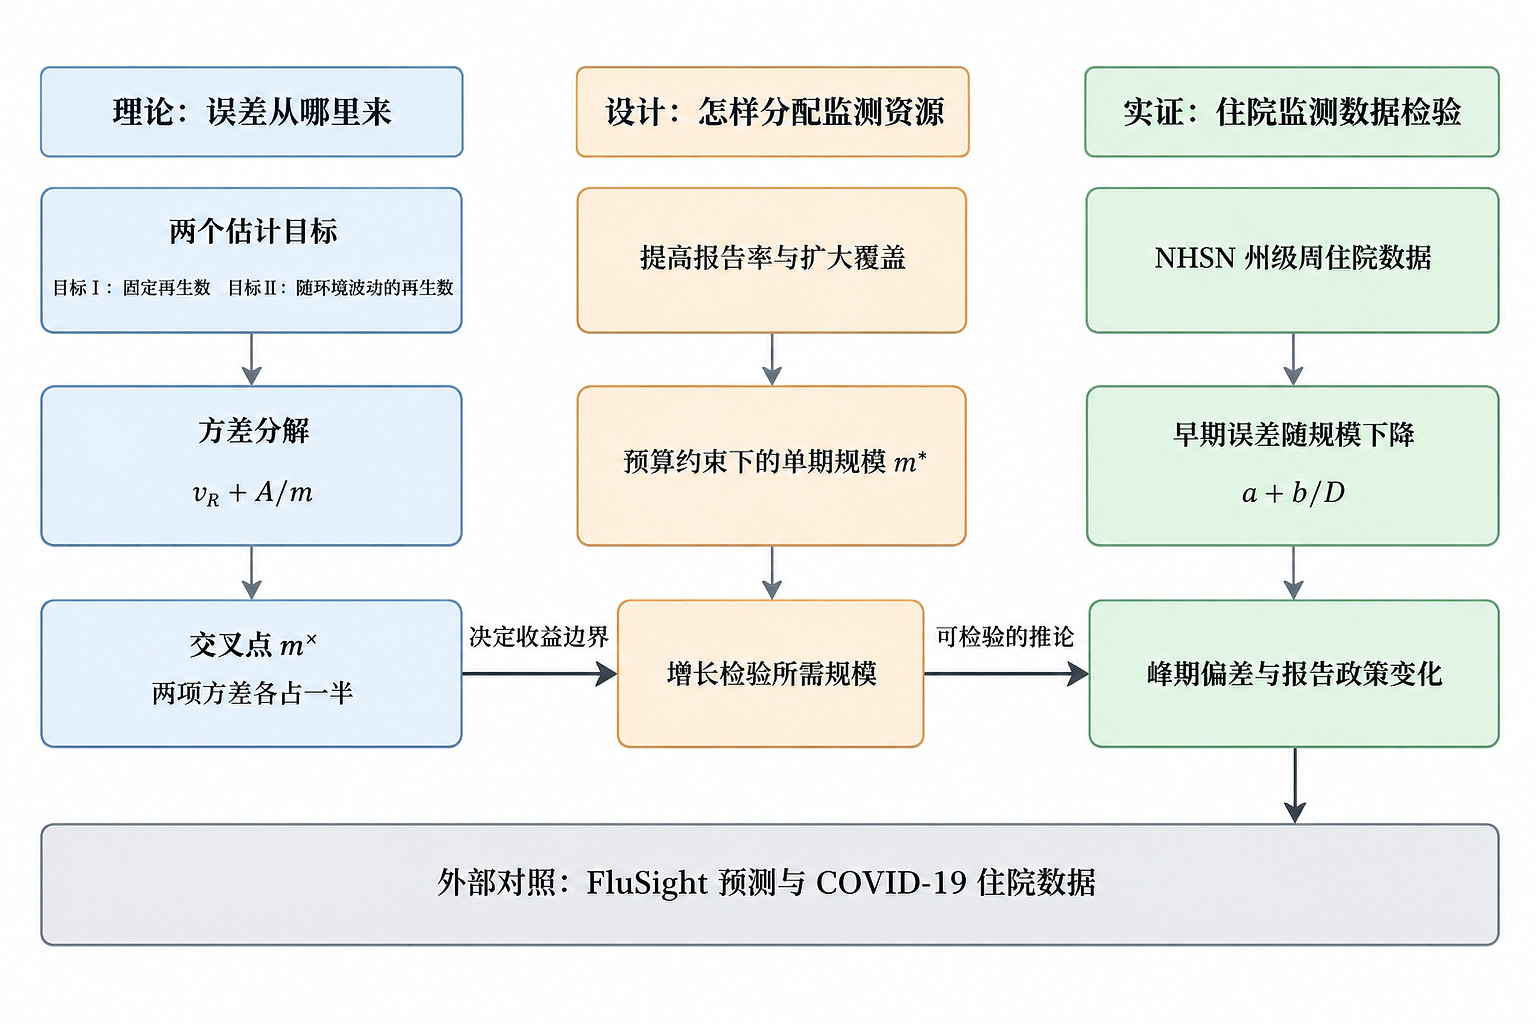
\includegraphics[width=\textwidth]{figures/fig_01_fig01_framework.pdf}
  \caption{本文结构。左列为方差理论，中列为由此得到的监测设计，右列为美国流感住院数据的检验，底部为外部对照。}
  \label{fig:framework}
\end{figure}
